\let\negmedspace\undefined
\let\negthickspace\undefined
\documentclass[journal]{IEEEtran}
\usepackage[a5paper, margin=10mm, onecolumn]{geometry}
%\usepackage{lmodern} % Ensure lmodern is loaded for pdflatex
\usepackage{tfrupee} % Include tfrupee package

\setlength{\headheight}{1cm} % Set the height of the header box
\setlength{\headsep}{0mm}     % Set the distance between the header box and the top of the text

\usepackage{gvv-book}
\usepackage{gvv}
\usepackage{cite}
\usepackage{amsmath,amssymb,amsfonts,amsthm}
\usepackage{algorithmic}
\usepackage{graphicx}
\usepackage{textcomp}
\usepackage{xcolor}
\usepackage{txfonts}
\usepackage{listings}
\usepackage{enumitem}
\usepackage{mathtools}
\usepackage{gensymb}
\usepackage{comment}
\usepackage[breaklinks=true]{hyperref}
\usepackage{tkz-euclide} 
\usepackage{listings}
% \usepackage{gvv}                                        
\def\inputGnumericTable{}                                 
\usepackage[latin1]{inputenc}                                
\usepackage{color}                                            
\usepackage{array}                                            
\usepackage{longtable}                                       
\usepackage{calc}                                             
\usepackage{multirow}                                         
\usepackage{hhline}                                           
\usepackage{ifthen}                                           
\usepackage{lscape}
\begin{document}

\bibliographystyle{IEEEtran}
\vspace{3cm}

\title{6.5.5.1}
\author{EE24BTECH11012 - Bhavanisankar G S}
% \maketitle
% \newpage
% \bigskip
{\let\newpage\relax\maketitle}

\renewcommand{\thefigure}{\theenumi}
\renewcommand{\thetable}{\theenumi}
\setlength{\intextsep}{10pt} % Space between text and floats


\numberwithin{equation}{enumi}
\numberwithin{figure}{enumi}
\renewcommand{\thetable}{\theenumi}

\textbf{QUESTION} : \\
Find the absolute maximum and minimum value of the function $f(x) = x^3$ in the interval $\sbrak{-2,2}$ \\
\textbf{SOLUTION} : \\

\textbf{Theoritical solution} : \\
Given function, 
\begin{align}
	y(x) &= x^3 \label{eq:fn} \\
	\implies y^{\prime} (x) &= 3 x^2  \label{eq:der} \\
	\implies y^{\prime \prime} (x) &= 6 x \label{eq:dder}
\end{align}
To find the critical points, we do
\begin{align}
	y^{\prime} (x) &= 0 \\
	3 x^2 &= 0 \\
	x &= 0 \label{eq:cp}
\end{align}
For 
\begin{align}
	Local min &\implies y^{\prime \prime} (x) > 0 \\
	Local max &\implies y^{\prime \prime} (x) < 0 \\
	Inflection point &\implies y^{\prime \prime} (x) = 0
\end{align}
Substituting \eqref{eq:cp} in \eqref{eq:dder}, we have
\begin{align}
	y^{\prime \prime} &= 0
\end{align}
Hence, \eqref{eq:cp} is a critical point. \\
Checking the edge values, we have \\
\begin{align}
	y(2) &= 8 \\
	y(-2) &= -8 \\
	y(0) &= 0
\end{align}
Hence, \\
\textbf{Absolute maximum} = 8 \\
\textbf{Absolute minimum} = -8 \\

\textbf{Computational solution} : \\

Finding maximum value of a function can be done using \textbf{Gradient Ascent method} \\
\begin{align}
	x_{n+1} &= x_{n} + \alpha f^{\prime} (x_{n}) \\
	x_{n+1} &= x_{n} + 3 \alpha x_{n}^2
\end{align}
Similarly, the minimum value can be found out using \textbf{Gradient descent} method. \\
\begin{align}
	x_{n+1} &= x_{n} - \alpha f^{\prime} (x_{n}) \\
	x_{n+1} &= x_{n} - 3 \alpha x_{n}^2
\end{align}
where $\alpha$ is the learning rate.
Taking
\begin{align}
	h &= 0.01 \\
	\alpha &= 0.01
\end{align}
we have
\begin{align}
	x_{min} &= -2 \\
	y_{min} &= -8 \\
	x_{max} &= 2 \\
	y_{max} &= 8
\end{align}

\begin{figure}[h]
\centering
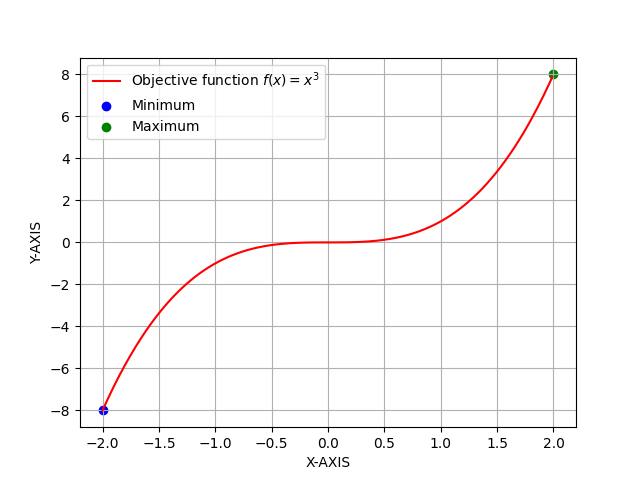
\includegraphics[width=\columnwidth]{figs/fig.png}
\caption{Plot of the given question.}
\label{fig:Plot1} 
\end{figure}
\end{document}
